% Experiment 5 checkpoint fragment. Not \input by the paper.
% Do not replace fig:exp2-k or fig:exp5-m.
% Each PDF has a 178 mm media box. Include at 178 mm.
% Paths are relative to this file.
% The lower row (NDCG@10) is an unsettled suggestion, not a second figure.
% Numbers are synthetic. Do not read a method advantage from them.

\begin{figure*}[t]
  \centering
  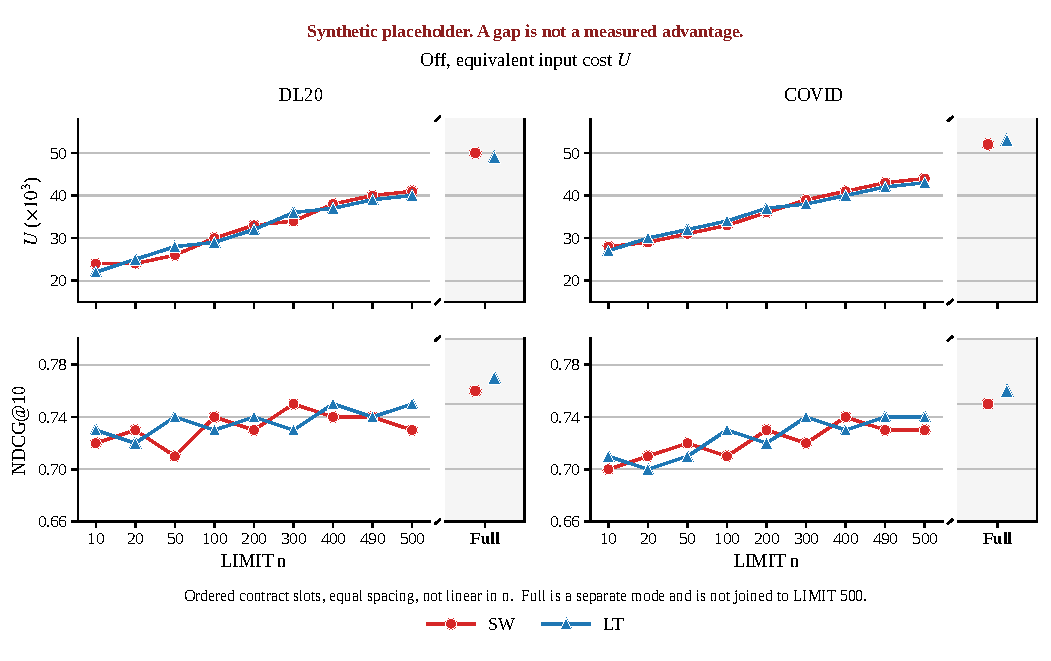
\includegraphics[width=178mm]{../figures/e5-limit-sweep-off.pdf}
  \caption{Off, synthetic placeholder for the LIMIT \(n\) contract
  \(10,20,50,100,200,300,400,490,500\).
  Slots are ordered and equally spaced; the spacing is not linear in \(n\).
  The last connected point is LIMIT 500 (buffer).
  Full is a separate mode in the broken-off band and is not joined to LIMIT 500.
  It is not \(K{=}510\).
  SW and LT use one marker each inside that band, shifted sideways only so the two marks stay distinct.
  The shift is not another observation.
  Cost is equivalent input \(U\) (\(\times 10^{3}\)).
  The lower row is NDCG@10 at every endpoint, including Full.
  This cost scale is not the On-cold scale.
  A gap is not a measured advantage.
  Qwen3.5-9B, \(n{=}500\), DL20 and COVID.
  These cells are not the equal-weight mean of three queries.}
  \label{fig:exp5-k-sweep-off}
\end{figure*}

\begin{figure*}[t]
  \centering
  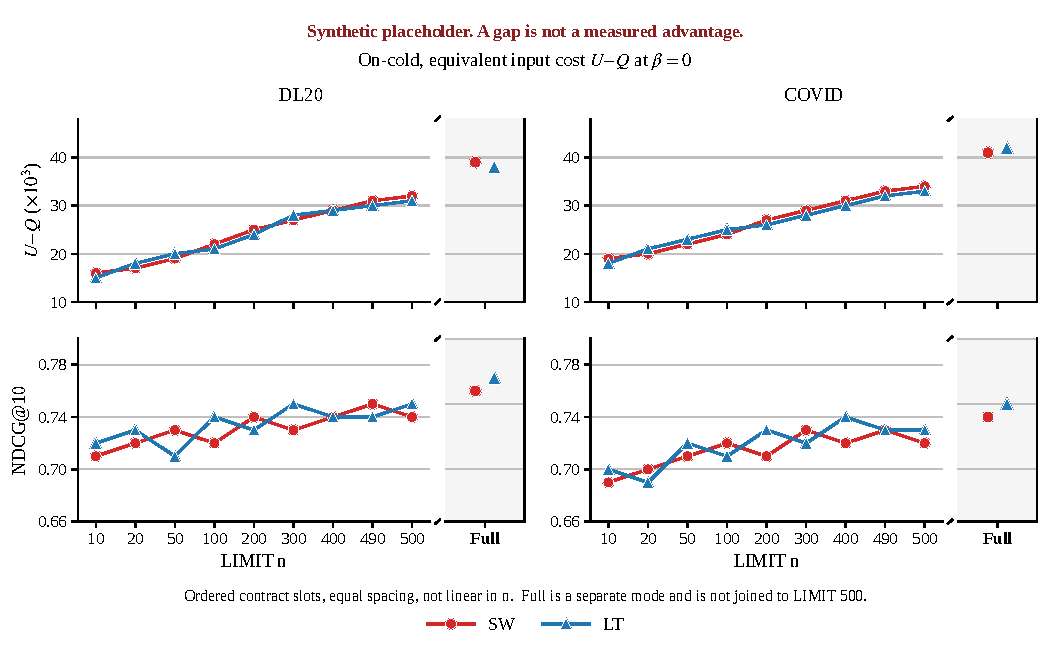
\includegraphics[width=178mm]{../figures/e5-limit-sweep-on.pdf}
  \caption{On-cold, same contract and same reading rules as \cref{fig:exp5-k-sweep-off}.
  Cost is \(U{-}Q\) at \(\beta{=}0\) (\(\times 10^{3}\)), on its own scale.
  NDCG@10 uses the same window as the Off figure.
  Synthetic placeholder. A gap is not a measured advantage.}
  \label{fig:exp5-k-sweep-on}
\end{figure*}
